\documentclass[11pt, a4paper]{article}

\usepackage{amsmath}
\usepackage{hyperref}
\usepackage{graphicx}
\usepackage{listings}
\usepackage{color}

\author{
  \textbf{KOTWAL ALANKAR SHASHIKANT}\\
  \texttt{12D070010}
  \and
  \textbf{ANAND KALVIT}\\
  \texttt{12D070032}
}
\title{Visual Odometry from Stereo Using Point-Set Matching}

\begin{document}
\maketitle
\newpage

\section{Introduction}
Odometry refers to the use of data from motion sensors to estimate change in position over time. One of the most reliable ways of estimation of 3-D structure using cameras is to use a calibrated stereo pair. Given the sequence of 3-D structures generated by the stereo camera, we can estimate the motion of the camera with respect to its environment as well as generate a 3-D map of the environment. This is usually referred to as visual SLAM (simultaneous localisation and mapping), which has wide applications in robotics and remote sensing. \\

\noindent We plan to implement a 6 DoF pose estimation algorithm using a calibrated stereo pair and generate a 3-D map of the environment simultaneously. We assume that scene illumination doesn't change much and most of the field of view of the camera is occupied by static parts of the environment. \\

\noindent In a nutshell, our job is to figure out what the translation and rotation of the camera is between two scenes as shown below. \\ \\ \\
\centerline{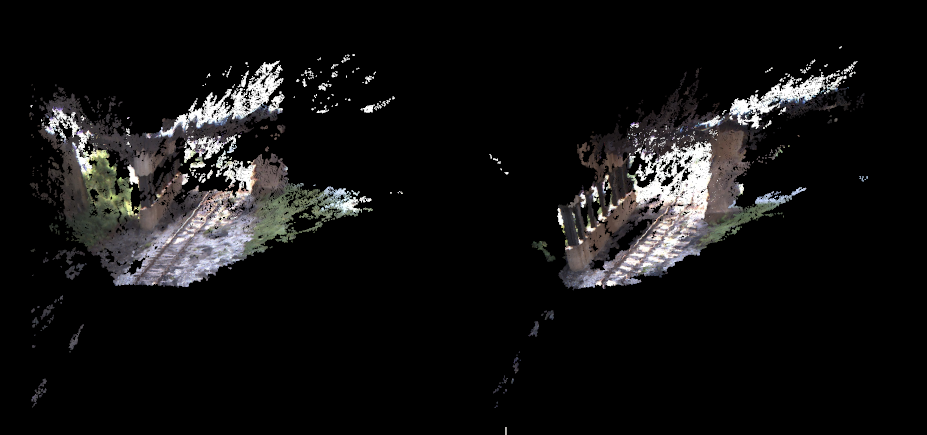
\includegraphics[scale=0.50]{pointclouds}}
\newpage

\section{Method}
We closely follow the method outlined in \cite{main}. The method involves modelling both the reference and the moving pointclouds as Mixture Models. We choose spherical Gaussian Mixtures and equal weights per-point for simplicity and easy updates. Our model for the pointclouds, thus, is given by $$\mathcal{S}(\textbf{x}) = \sum_{i=1}^N \mathcal{G}(\textbf{x}; \textbf{s}_i, \Sigma), \mathcal{M}(\textbf{x}) = \sum_{i=1}^M \mathcal{G}(\textbf{x}; \textbf{m}_i, \Sigma)$$ where $N = |\mathcal{S}|, M = |\mathcal{M}|, \Sigma = diag(\sigma^2)$. We then maximise the kernel correlation between a translated and rotated version of the moving pointcloud and the reference pointcloud, with respect to the rotation and the translation, yielding the optimization problem $$\min_{\textbf{R}, \textbf{t}} \sum_{i=1}^M \sum_{j=1}^N e^{-\frac{|| \textbf{d}_{ij} ||}{2 \sigma^2}}$$ such that $\textbf{d}_{ij} = \textbf{Rx}_i + \textbf{t} - \textbf{y}_j$ and $\textbf{R}^T \textbf{R} = I$. This is a convex program and the optimization is carried out using Gradient Descent on the components of $\textbf{t}$ and a parametrization of the rotation matrix $\textbf{R}$, as described in the implementation section below.

\section{Implementation}

\section{Results}


\begin{thebibliography}{9}

\bibitem{main}
  Bing Jian and Vemuri, B.C.,
  \emph{Robust Point Set Registration Using Gaussian Mixture Models}.
  IEEE Transactions on Pattern Analysis and Machine Intelligence,
  2010.
  
\bibitem{mainPre}
  Pre-print of the above paper \href{http://code.google.com/p/gmmreg/downloads/detail?name=gmmreg_PAMI_preprint.pdf}{here}.
  
\bibitem{quatParam}
  George Terzakis, Phil Culverhouse \textit{et al},
  \emph{A Recipe on the Parameterization of Rotation Matrices for Non-Linear Optimization using Quaternions}.
  Technical Report of the School of Marine Science and Engineering, Plymouth University,
  2012.
  
\bibitem{cppStuff}
  Documentation for the OpenCV, Point Cloud and Eigen libraries in C++ \href{http://docs.opencv.org/}{here}, \href{http://pointclouds.org/documentation/}{here} and \href{http://eigen.tuxfamily.org/dox/}{here} respectively

\end{thebibliography}

\end{document}